

\documentclass[crop,tikz]{standalone}% 'crop' is the default for v1.0, before it was 'preview'
\usepackage{pgfplots}
\pgfplotsset{compat=newest}
\usetikzlibrary{calc}
\usetikzlibrary{shapes.geometric}
\usetikzlibrary{decorations.pathreplacing,calligraphy}
\usetikzlibrary{shapes,arrows,chains}

\begin{document}
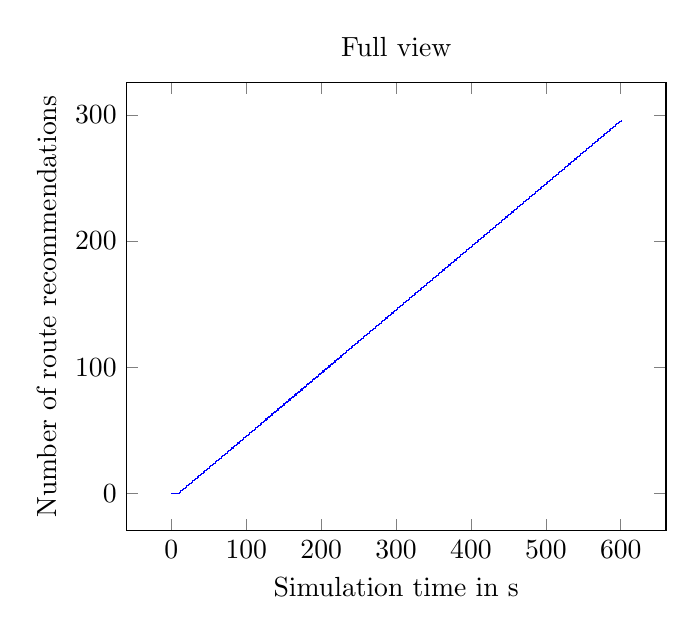
\begin{tikzpicture}
\begin{axis}[xlabel=Simulation time in s,ylabel=Number of route recommendations, title=Full view]
\addplot+ [no marks,const plot mark left] table [x=Time,y=Number] {
Time Number
0.0  0
10.4 1
12.4 2
14.4 3
16.4 4
18.4 5
20.4 6
22.4 7
24.4 8
26.4 9
28.4 10
30.4 11
32.4 12
34.4 13
36.4 14
38.4 15
40.4 16
42.4 17
44.4 18
46.4 19
48.4 20
50.4 21
52.4 22
54.4 23
56.4 24
58.4 25
60.4 26
62.4 27
64.4 28
66.4 29
68.4 30
70.4 31
72.4 32
74.4 33
76.4 34
78.4 35
80.4 36
82.4 37
84.4 38
86.4 39
88.4 40
90.4 41
92.4 42
94.4 43
96.4 44
98.4 45
100.4 46
102.4 47
104.4 48
106.4 49
108.4 50
110.4 51
112.4 52
114.4 53
116.4 54
118.4 55
120.4 56
122.4 57
124.4 58
126.4 59
128.4 60
130.4 61
132.4 62
134.4 63
136.4 64
138.4 65
140.4 66
142.4 67
144.4 68
146.4 69
148.4 70
150.4 71
152.4 72
154.4 73
156.4 74
158.4 75
160.4 76
162.4 77
164.4 78
166.4 79
168.4 80
170.4 81
172.4 82
174.4 83
176.4 84
178.4 85
180.4 86
182.4 87
184.4 88
186.4 89
188.4 90
190.4 91
192.4 92
194.4 93
196.4 94
198.4 95
200.4 96
202.4 97
204.4 98
206.4 99
208.4 100
210.4 101
212.4 102
214.4 103
216.4 104
218.4 105
220.4 106
222.4 107
224.4 108
226.4 109
228.4 110
230.4 111
232.4 112
234.4 113
236.4 114
238.4 115
240.4 116
242.4 117
244.4 118
246.4 119
248.4 120
250.4 121
252.4 122
254.4 123
256.4 124
258.4 125
260.4 126
262.4 127
264.4 128
266.4 129
268.4 130
270.4 131
272.4 132
274.4 133
276.4 134
278.4 135
280.4 136
282.4 137
284.4 138
286.4 139
288.4 140
290.4 141
292.4 142
294.4 143
296.4 144
298.4 145
300.4 146
302.4 147
304.4 148
306.4 149
308.4 150
310.4 151
312.4 152
314.4 153
316.4 154
318.4 155
320.4 156
322.4 157
324.4 158
326.4 159
328.4 160
330.4 161
332.4 162
334.4 163
336.4 164
338.4 165
340.4 166
342.4 167
344.4 168
346.4 169
348.4 170
350.4 171
352.4 172
354.4 173
356.4 174
358.4 175
360.4 176
362.4 177
364.4 178
366.4 179
368.4 180
370.4 181
372.4 182
374.4 183
376.4 184
378.4 185
380.4 186
382.4 187
384.4 188
386.4 189
388.4 190
390.4 191
392.4 192
394.4 193
396.4 194
398.4 195
400.4 196
402.4 197
404.4 198
406.4 199
408.4 200
410.4 201
412.4 202
414.4 203
416.4 204
418.4 205
420.4 206
422.4 207
424.4 208
426.4 209
428.4 210
430.4 211
432.4 212
434.4 213
436.4 214
438.4 215
440.4 216
442.4 217
444.4 218
446.4 219
448.4 220
450.4 221
452.4 222
454.4 223
456.4 224
458.4 225
460.4 226
462.4 227
464.4 228
466.4 229
468.4 230
470.4 231
472.4 232
474.4 233
476.4 234
478.4 235
480.4 236
482.4 237
484.4 238
486.4 239
488.4 240
490.4 241
492.4 242
494.4 243
496.4 244
498.4 245
500.4 246
502.4 247
504.4 248
506.4 249
508.4 250
510.4 251
512.4 252
514.4 253
516.4 254
518.4 255
520.4 256
522.4 257
524.4 258
526.4 259
528.4 260
530.4 261
532.4 262
534.4 263
536.4 264
538.4 265
540.4 266
542.4 267
544.4 268
546.4 269
548.4 270
550.4 271
552.4 272
554.4 273
556.4 274
558.4 275
560.4 276
562.4 277
564.4 278
566.4 279
568.4 280
570.4 281
572.4 282
574.4 283
576.4 284
578.4 285
580.4 286
582.4 287
584.4 288
586.4 289
588.4 290
590.4 291
592.4 292
594.4 293
596.4 294
598.4 295
600.4 296
};
\end{axis}
\end{tikzpicture}
\end{document}